
%(BEGIN_QUESTION)
% Copyright 2007, Tony R. Kuphaldt, released under the Creative Commons Attribution License (v 1.0)
% This means you may do almost anything with this work of mine, so long as you give me proper credit

Shown here is the response of a process to a series of step-changes on the controller output (all made with the controller in ``manual'' mode).  Based on your observations, what can you ascertain about the process and its related instrumentation?

$$\includegraphics[width=15.5cm]{i01649x01.eps}$$

\underbar{file i01649}
%(END_QUESTION)





%(BEGIN_ANSWER)

This plot of PV response for several step-changes in output shows the process to possess a significant amount of {\it hysteresis}.  If this is a process controlled by a valve, I would suspect that the valve had significant "stiction" and/or looseness in a mechanical coupling.

Note how the first upward output step-change has no measurable effect on the process variable.  But on the second and third upward step-changes, the process variable responds immediately with upward jumps.  Likewise, on the first downward output step-change, there is no measurable effect on the process variable.  However, the process responds swiftly to the second and third downward output step-changes.  In summary, we see no effect on the first output reversal-of-direction.  This is characteristic of {\it hysteresis}, wherever it may reside in the system.  The most likely source of this hysteresis is in the control valve (stiction).

%(END_ANSWER)





%(BEGIN_NOTES)

%INDEX% Control, PID tuning: step change (output) revealing hysteresis

%(END_NOTES)


